\section{Валидация алгоритмов и сравнение алгоритмов. Задача выбора алгоритма.}

\D{
    Валидация = вычисление $L(A, D)$ по $L_D(a_\theta)$

    Тестирование на множестве $D$ = вычисление $L_D(a_\theta)$
    из $L(\hat{y}, y)$

    Инференс = вычисление $a_\theta(x)$

    Бывает:
    \begin{itemize}
        \item Hold-out validation
        \item Cross validation
    \end{itemize}
}

Нет абсолютного критерия сравнения алгоритмов. Нужно зафиксировать
набор данных, функцию ошибки и методику вычисления.

\T[NoFreeLunch]{
    Если алгоритм хорошо работает на определенном множестве
    наборов данных, то это скажется на производительности на 
    множестве всех оставшихся наборов данных.

    \begin{proof}
        По набору данных строим новый набор, где в тестовой
        части инвертируем метки классов.

        Получаем, что качество $q_2 = 1 - q_2$ и неравенство
        на качество алгоритмов обучения инвертируется.
    \end{proof}
}

Выбор алгоритма для набора данных относительно ошибки:
$A_{best} = \arg \min_A L(A, D)$

% \begin{figure}[H]
% 	\centering
% 	\begin{minipage}[b]{0.4\textwidth}
% 		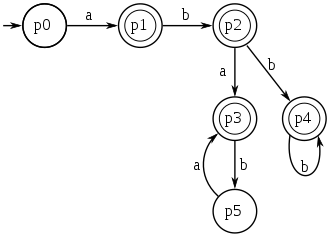
\includegraphics[width=\textwidth]{images/dfa.png}
% 		\caption{Пример графа переходов детерминированного КА.}
% 	\end{minipage}
% 	\hfill
% 	\begin{minipage}[b]{0.4\textwidth}
% 		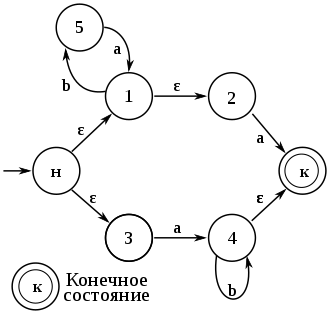
\includegraphics[width=\textwidth]{images/ndfa.png}
% 		\caption{Пример графа переходов недетерминированного КА с самопроизвольными переходами.}
% 	\end{minipage}
% \end{figure}